%
% compile with pdflatex:
%   $ pdflatex homework-hw
% , yields homework-example.pdf
%    You might need to compile twice, if, e.g., you start using references
%

\documentclass[10pt,letterpaper,oneside]{article}
\usepackage[ascii]{inputenc}
\usepackage{graphicx}
\graphicspath{ {} }
\usepackage{amsmath,amsfonts,amssymb}
\usepackage{parselines} 
\usepackage[margin=1in]{geometry}
	\setlength{\parindent}{0em}
	\setlength{\parskip}{1em}



\newtheorem{theorem}{Theorem}

%%%% user definitions %%%%%%%%%%%%%%%%%%%%%%%

\newcommand{\Problem}[1]{\subsection*{Problem #1}}
\newcommand{\Part}[1]{\subsubsection*{Part #1}}
\newcommand{\Solution}{\subsubsection*{Solution}}

	% Forms for Big-Oh notation
\DeclareMathOperator{\Omicron}{O}
\DeclareMathOperator{\omicron}{o}

\newcommand{\BigOh}[1]{\Omicron(#1)}
\newcommand{\LittleOh}[1]{\omicron(#1)}
\newcommand{\BigOmega}[1]{\Omega(#1)}
\newcommand{\LittleOmega}[1]{\omega(#1)}
\newcommand{\BigTheta}[1]{\Theta(#1)}

	% Operators for dominance notation
\newcommand{\domeq}{\sim}
\newcommand{\domle}{\preceq}
\newcommand{\domlt}{\prec}
\newcommand{\domge}{\succeq}
\newcommand{\domgt}{\succ}

\newcommand\tab[1][1cm]{\hspace*{#1}}


%%%%%%%%  You edit stuff below this line  %%%%%%%%%%%%%%%%%%%%%%%%%%

\title{HW9 Theory}
\author{Alexander Kazantsev}
%\date{}  % uses today, by default

\begin{document}
\maketitle
\Problem{6.2}
If each $T_i$ is a vertex, and the direction of the graph points to each $T_i$ that needs completion before $T_j$ DFS can be leveraged. First DFS on each vertex should be computed, with each set generated off of each vertex used as a reference for every other vertex referencing that set. This will generate at minimum one topologically ordered set, or at maximum $T_n$ sets. Each set should be walked backwards, with their times $t_i$ summed. 
\Problem{6.8}
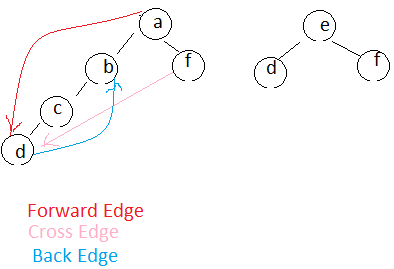
\includegraphics{forest.png}
\Problem{6.10}

CountDepth( G, r )

	\tab label r as discovered

	\tab count = 1

	\tab for all edges from v to w in G.adjacentEdges( r )

	\tab \tab if w not discovered

	\tab \tab \tab count += CountDepth( G, w)

	\tab return count

IsRooted ( G )
	
	\tab for all v in G.vertices

	\tab \tab result = CountDepth( G, v )

	\tab \tab if result == length( G.verticies )

	\tab \tab \tab return true

	\tab return false
	
\Problem{6.14}

under the assumption that the paths are unweighted

Time complexity is $ v^2 + v*e$

Paths( G, v,paths = [ ] )
	
	\tab result = [ ]

	\tab for e in G[v].edges

	\tab \tab result.append( Paths(G, e, paths + [ v ] ) )

	\tab return result

LongestPath( G )

	\tab result = [ ]	

	\tab for v in G.vertices
	
	\tab \tab result.append( Paths( G, v ) )

	\tab return max( result )
\Problem{6.15}
(f,d,b,c)

\Problem{6.20}
too late to write this algo, but it should utilize DFS
\Problem{7.3}
\Part{c}
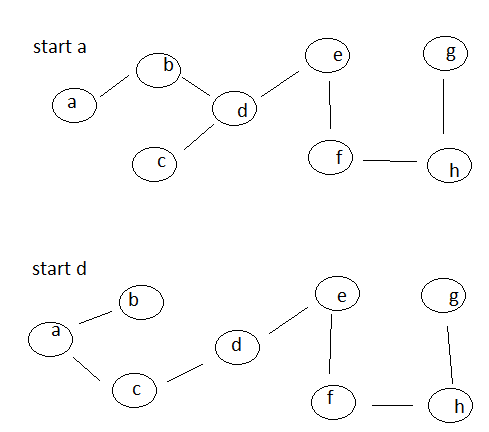
\includegraphics{trees.png}
\maketitle
\end{document}